%%%%%%%%%%%%%%%%%%%%%%%%%%%%%%%%%%%%%%%%%
% Journal Article
% LaTeX Template
% Version 2.0 (February 7, 2023)
%
% This template originates from:
% https://www.LaTeXTemplates.com
%
% Author:
% Vel (vel@latextemplates.com)
%
% License:
% CC BY-NC-SA 4.0 (https://creativecommons.org/licenses/by-nc-sa/4.0/)
%
% NOTE: The bibliography needs to be compiled using the biber engine.
%
%%%%%%%%%%%%%%%%%%%%%%%%%%%%%%%%%%%%%%%%%

%----------------------------------------------------------------------------------------
%	PACKAGES AND OTHER DOCUMENT CONFIGURATIONS
%----------------------------------------------------------------------------------------

\documentclass[
	a4paper, % Paper size, use either a4paper or letterpaper
	10pt, % Default font size, can also use 11pt or 12pt, although this is not recommended
	%unnumberedsections, % Comment to enable section numbering
	twoside, % Two side traditional mode where headers and footers change between odd and even pages, comment this option to make them fixed
]{LTJournalArticle}

\addbibresource{sample.bib} % BibLaTeX bibliography file

\runninghead{} % A shortened article title to appear in the running head, leave this command empty for no running head

\footertext{} % Text to appear in the footer, leave this command empty for no footer text

\setcounter{page}{1} % The page number of the first page, set this to a higher number if the article is to be part of an issue or larger work

%----------------------------------------------------------------------------------------
%	TITLE SECTION
%----------------------------------------------------------------------------------------

\title{Modelling Cognition} % Article title, use manual lines breaks (\\) to beautify the layout

% Authors are listed in a comma-separated list with superscript numbers indicating affiliations
% \thanks{} is used for any text that should be placed in a footnote on the first page, such as the corresponding author's email, journal acceptance dates, a copyright/license notice, keywords, etc
\author{%
	Matthew Hinton\textsuperscript{1}\thanks{Corresponding author: \href{mailto:matthewhinton@uvic.ca}{matthewhinton@uvic.ca}} and Preston Pan\textsuperscript{2}\thanks{Corresponding author: \href{mailto:preston@nullring.xyz}{preston@nullring.xyz}}\\ March, 2024
	% {Corresponding author: \href{mailto:preston@nullring.xyz}{preston@nullring.xyz}\\ \textbf{Date:} March, 2024}
}

% Affiliations are output in the \date{} command
\date{\footnotesize\textsuperscript{\textbf{1}}University of Victoria}

% Full-width abstract
\renewcommand{\maketitlehookd}{%
	\begin{abstract}
          \noindent
          Cognition is a system wherein components of the language are public to the language itself. It is written
          in pure postfix notation, and removes the prefix characteristics of other similar languages.
          This enables the Cognition interpreter to be able to manipulate its state based on code read on the fly
          in a token stream, giving it the property of tokenizing and parsing future characters differently than it does
          current characters. The result is an unopinionated language that can replicate a wide variety of different
          syntaxes, allowing Cognition to modify syntax entirely during runtime. This paper investigates the implications
          of this programming language, which has potential applications in parsing and self-modifying systems.
        \end{abstract}
}

%----------------------------------------------------------------------------------------

\begin{document}

\maketitle % Output the title section

%----------------------------------------------------------------------------------------
%	ARTICLE CONTENTS
%----------------------------------------------------------------------------------------

\section{Introduction}
Current programming languages operate with parsing requirements. This means that the parser must read ahead
of the current token to decide what to do with the current token being passed into the parser. This usually causes
the langauge to have a static syntax, due to the parser being too rigid for the AST to be made public. Metaprogramming
languages solve this problem by making parts of the AST public, and in particular, concatenative programming languages such
as forth, factor, and stem solve a part of this problem by introducing postfix notation for symbols usually known as \emph{words},
which reduce the need for parsing by allowing tokens to be evaluated one-at-a-time. Many of these languages then utilize
metaprogramming in order to alter the execution order of the tokens, usually using quotes.
However, they don't remove the requirement of \emph{reading ahead}. Instead, they outsource this process to quotes,
which are required for turing completeness in the form of recursion. Worse, many of these languages have strings, which
require the parser or tokenizer to read ahead in order to package the string as a single token. Therefore, many of these
languages are not perfect candidates for a perfectly postfix language.

Cognition solves this problem using three mechanisms: first, tokens are one character long by default and information
about how Cognition will tokenize based on certain delimiter rules are made public to the language; second, Cognition
uses a unique metacrank system which allows it to modify the execution order of the code, allowing Cognition to
\emph{modify the syntax for changing the execution order itself} due to the metacrank system's postfix syntax, and allow
for metaprogramming; third, it uses what we call an \emph{falias} system which we believe to be equivalent to metacrank, but makes
for easier bootstrapping to an environment that is more desirable to program in.


%------------------------------------------------

\section{Language Design}
As of the release of this paper, the language design is incomplete yet still covers many general cases. Tradeoffs
in the implementation have been made such that the esscence of the design is there but the implementation is simplified.
In this section, we describe the high level overview of the public components of Cognition, and we compare and contrast
it with other similarly flexible programming languages such as Forth and Lisp.

In languages like lisp and forth, syntax can be modified using \emph{macros}. The usage of macros allows for the publicity
of the AST; that is, it allows for the change in execution order of symbols or words. Similarily, Cognition allows for this
behavior, by using a \emph{metacranking} system, which allows it to specify every \emph{nth} word \emph{n} items down the
stack to be executed, where all the other words are not evaluated. Metacranking behavior can be modified using a postfix
syntax, allowing metacrank execution order itself to be changed, meaning not only can the AST be modified, but the system
used to modify the AST is itself a part of the AST and can be modified. This allows full AST modification, and we believe
it to not be possible with many more naive implementations of Forth and many, if not all implementations of Lisp.

Because everything is written in postfix notation, there is almost no need for a special character that denotes the AST
like in the case with the parentheses in Lisp. Instead, there is an falias system which force evaluates the top item
on the stack in a \emph{fast} way, without waiting for the cranker. It is conceptually possible to modify the bracket
syntax for lisp and for Forth, but it is unwieldy due to its prefix nature.

This gives Cognition the benefit of never reading ahead. Because it never has to read more characters than it has to, only obeying
a couple of delimiter, ignored character, and singlet laws, it allows the tokenization strategy of the parser to be changed
without affecting the current token or future tokens in unwanted or conflicting ways. This allows other special characters
that denote the delimiter between different tokens, for example, to be made public, and allows them to therefore be changed
dynamically and programmatically, giving even more power to the AST manipulation as operations modifying the tokenizer can be
stored in the stack and changed via the metacranker. Furthermore, string operations in Cognition modify the tokens
post-tokenization, making post tokenization decisions about token execution possible.

The hash table that stores variable definitions is also made public, allowing the program to access currently defined variables,
modify them, and delete them. This principle is made more powerful with metastack operations which have the main focus of
reducing the possibility of hash table collisions and making program simulation and program introspection easy.

Metastack operations extend the definition of Forth quotes, attaching a hash table and other data structures required to make
a complete cognition environment to quotes, making them self similar to the original environment. This is important for
implementing scope, containerization, and self-simulation. This allows Cognition to be used as a permission system in a
Cognition-centric virtual machine or operating system in the future.

Otherwise, Cognition is much like the programming language forth, with a stack-based postfix programming environment.
\subsection{Parser Design}
The parser is designed to make public the specifics of how characters are parsed into tokens by delimiter rules,
and by a few other constructs called \emph{ignores} and \emph{singlets}. Ignores allow the parser to ignore a list
of characters at the start of the read-eval-print loop, and delimiters and singlets allow the parser to determine
the end of the next token.

The parser has three flags for these features, where the flags represent the decision to whitelist or blacklist
the characters to be ignored, or to be singlets or delimiters that stop the parser from collecting the token.
When the parser hits a delimiter, the parser stops and the token gets packaged, whereas when the parser hits
a singlet, the parser skips the singlet character. This enables a wide range of source file text manipulation.
If characters were not ignored, at least one character must be parsed into a word, and if not, a word containing
no characters can be created with singlets.

By default, the parser starts with no ignored characters, no blacklisted delimiters (everything is a delimiter), and no
singlets.
\subsection{Falias Design}
Force aliases, or faliases for short, are a list of special tokens that evaluate the top word on the stack unconditionally
when tokenized. One can change the list of faliases and one can even make the list empty, effectively removing the falias
functionality.

By default, \emph{f} is the only falias.
\subsection{Metacrank Design}
The metacranker is a cyclic automatic word evaluation system, where \emph{cranking} refers to metacranking the first
element on the stack, meaning that the top element of the stack executes once every \emph{n} words executed. \emph{Metacranking}
refers to the mth element down the current stack executing once every \emph{n} words executed. There can only be one word
executed every crank, although all metacrank positions are incremented every cycle. Therefore, the top of the stack executes
first, and the highest metacrank has the lowest priority, executing only if every other crank above doesn't execute.

There are two kinds of words that can be evaluated: macros, and definitions. Macros
The metacrank default is set to zero, which you can take to represent an infinite crank cycle (it doesn't make sense to talk
about a zero metacrank base otherwise). In this state, the only way one can execute words is using the \emph{falias} system.
However, one can quickly set a crank and get into a comfortable environment without having to use faliases.
\subsection{Metastack Design}
The metastack is a system by which the current working stack can be set. Each current working stack has a hash table associated
and an error stack associated,
\subsection{Error Stack Design}

\subsection{Builtins and the FLIT}

This line shows how to use a footnote to further explain or cite text\footnote{Example footnote text.}.

This is a bullet point list:

\begin{itemize}
	\item Arcu eros accumsan lorem, at posuere mi diam sit amet tortor
	\item Fusce fermentum, mi sit amet euismod rutrum
	\item Sem lorem molestie diam, iaculis aliquet sapien tortor non nisi
	\item Pellentesque bibendum pretium aliquet
\end{itemize}

Mauris interdum porttitor fringilla. Proin tincidunt sodales leo at ornare. Donec tempus magna non mauris gravida luctus. Cras vitae arcu vitae mauris eleifend scelerisque. Nam sem sapien, vulputate nec felis eu, blandit convallis risus. Pellentesque sollicitudin venenatis tincidunt. In et ipsum libero. Nullam tempor ligula a massa convallis pellentesque.

This is a numbered list:

\begin{enumerate}
	\item Donec dolor arcu, rutrum id molestie in, viverra sed diam
	\item Curabitur feugiat
	\item Turpis sed auctor facilisis
\end{enumerate}

\subsection{Species Identification}

Proin lobortis efficitur dictum. Pellentesque vitae pharetra eros, quis dignissim magna. Sed tellus leo, semper non vestibulum vel, tincidunt eu mi. Aenean pretium ut velit sed facilisis. Ut placerat urna facilisis dolor suscipit vehicula. Ut ut auctor nunc. Nulla non massa eros. Proin rhoncus arcu odio, eu lobortis metus sollicitudin eu. Duis maximus ex dui, id bibendum diam dignissim id. Aliquam quis lorem lorem. Phasellus sagittis aliquet dolor, vulputate cursus dolor convallis vel. Suspendisse eu tellus feugiat, bibendum lectus quis, fermentum nunc. Nunc euismod condimentum magna nec bibendum. Curabitur elementum nibh eu sem cursus, eu aliquam leo rutrum. Sed bibendum augue sit amet pharetra ullamcorper. Aenean congue sit amet tortor vitae feugiat.

Mauris interdum porttitor fringilla. Proin tincidunt sodales leo at ornare. Donec tempus magna non mauris gravida luctus. Cras vitae arcu vitae mauris eleifend scelerisque. Nam sem sapien, vulputate nec felis eu, blandit convallis risus. Pellentesque sollicitudin venenatis tincidunt. In et ipsum libero. Nullam tempor ligula a massa convallis pellentesque.

\subsection{Data Analysis}

Vestibulum sodales orci a nisi interdum tristique. In dictum vehicula dui, eget bibendum purus elementum eu. Pellentesque lobortis mattis mauris, non feugiat dolor vulputate a. Cras porttitor dapibus lacus at pulvinar. Praesent eu nunc et libero porttitor malesuada tempus quis massa. Aenean cursus ipsum a velit ultricies sagittis. Sed non leo ullamcorper, suscipit massa ut, pulvinar erat. Aliquam erat volutpat. Nulla non lacus vitae mi placerat tincidunt et ac diam. Aliquam tincidunt augue sem, ut vestibulum est volutpat eget. Suspendisse potenti. Integer condimentum, risus nec maximus elementum, lacus purus porta arcu, at ultrices diam nisl eget urna. Curabitur sollicitudin diam quis sollicitudin varius. Ut porta erat ornare laoreet euismod. In tincidunt purus dui, nec egestas dui convallis non. In vestibulum ipsum in dictum scelerisque.

Mauris interdum porttitor fringilla. Proin tincidunt sodales leo at ornare. Donec tempus magna non mauris gravida luctus. Cras vitae arcu vitae mauris eleifend scelerisque. Nam sem sapien, vulputate nec felis eu, blandit convallis risus. Pellentesque sollicitudin venenatis tincidunt. In et ipsum libero. Nullam tempor ligula a massa convallis pellentesque. Mauris interdum porttitor fringilla. Proin tincidunt sodales leo at ornare. Donec tempus magna non mauris gravida luctus. Cras vitae arcu vitae mauris eleifend scelerisque. Nam sem sapien, vulputate nec felis eu, blandit convallis risus. Pellentesque sollicitudin venenatis tincidunt. In et ipsum libero. Nullam tempor ligula a massa convallis pellentesque.

%------------------------------------------------

\section{Results}

\begin{table} % Single column table
	\caption{Example single column table.}
	\centering
	\begin{tabular}{l l r}
		\toprule
		\multicolumn{2}{c}{Location} \\
		\cmidrule(r){1-2}
		East Distance & West Distance & Count \\
		\midrule
		100km & 200km & 422 \\
		350km & 1000km & 1833 \\
		600km & 1200km & 890 \\
		\bottomrule
	\end{tabular}
	\label{tab:distcounts}
\end{table}

Referencing a table using its label: Table \ref{tab:distcounts}.

\begin{table*} % Full width table (notice the starred environment)
	\caption{Example two column table with fixed-width columns.}
	\centering % Horizontally center the table
	\begin{tabular}{L{0.2\linewidth} L{0.2\linewidth} R{0.15\linewidth}} % Manually specify column alignments with L{}, R{} or C{} and widths as a fixed amount, usually as a proportion of \linewidth
		\toprule
		\multicolumn{2}{c}{Location} \\
		\cmidrule(r){1-2}
		East Distance & West Distance & Count \\
		\midrule
		100km & 200km & 422 \\
		350km & 1000km & 1833 \\
		600km & 1200km & 890 \\
		\bottomrule
	\end{tabular}
\end{table*}

Aenean feugiat pellentesque venenatis. Sed faucibus tristique tortor vel ultrices. Donec consequat tellus sapien. Nam bibendum urna mauris, eget sagittis justo gravida vel. Mauris nisi lacus, malesuada sit amet neque ut, venenatis tempor orci. Curabitur feugiat sagittis molestie. Duis euismod arcu vitae quam scelerisque facilisis. Praesent volutpat eleifend tortor, in malesuada dui egestas id. Donec finibus ac risus sed pellentesque. Donec malesuada non magna nec feugiat. Mauris eget nibh nec orci congue porttitor vitae eu erat. Sed commodo ipsum ipsum, in elementum neque gravida euismod. Cras mi lacus, pulvinar ut sapien ut, rutrum sagittis dui. Donec non est a metus varius finibus. Pellentesque rutrum pellentesque ligula, vitae accumsan nulla hendrerit ut.

\begin{figure} % Single column figure
	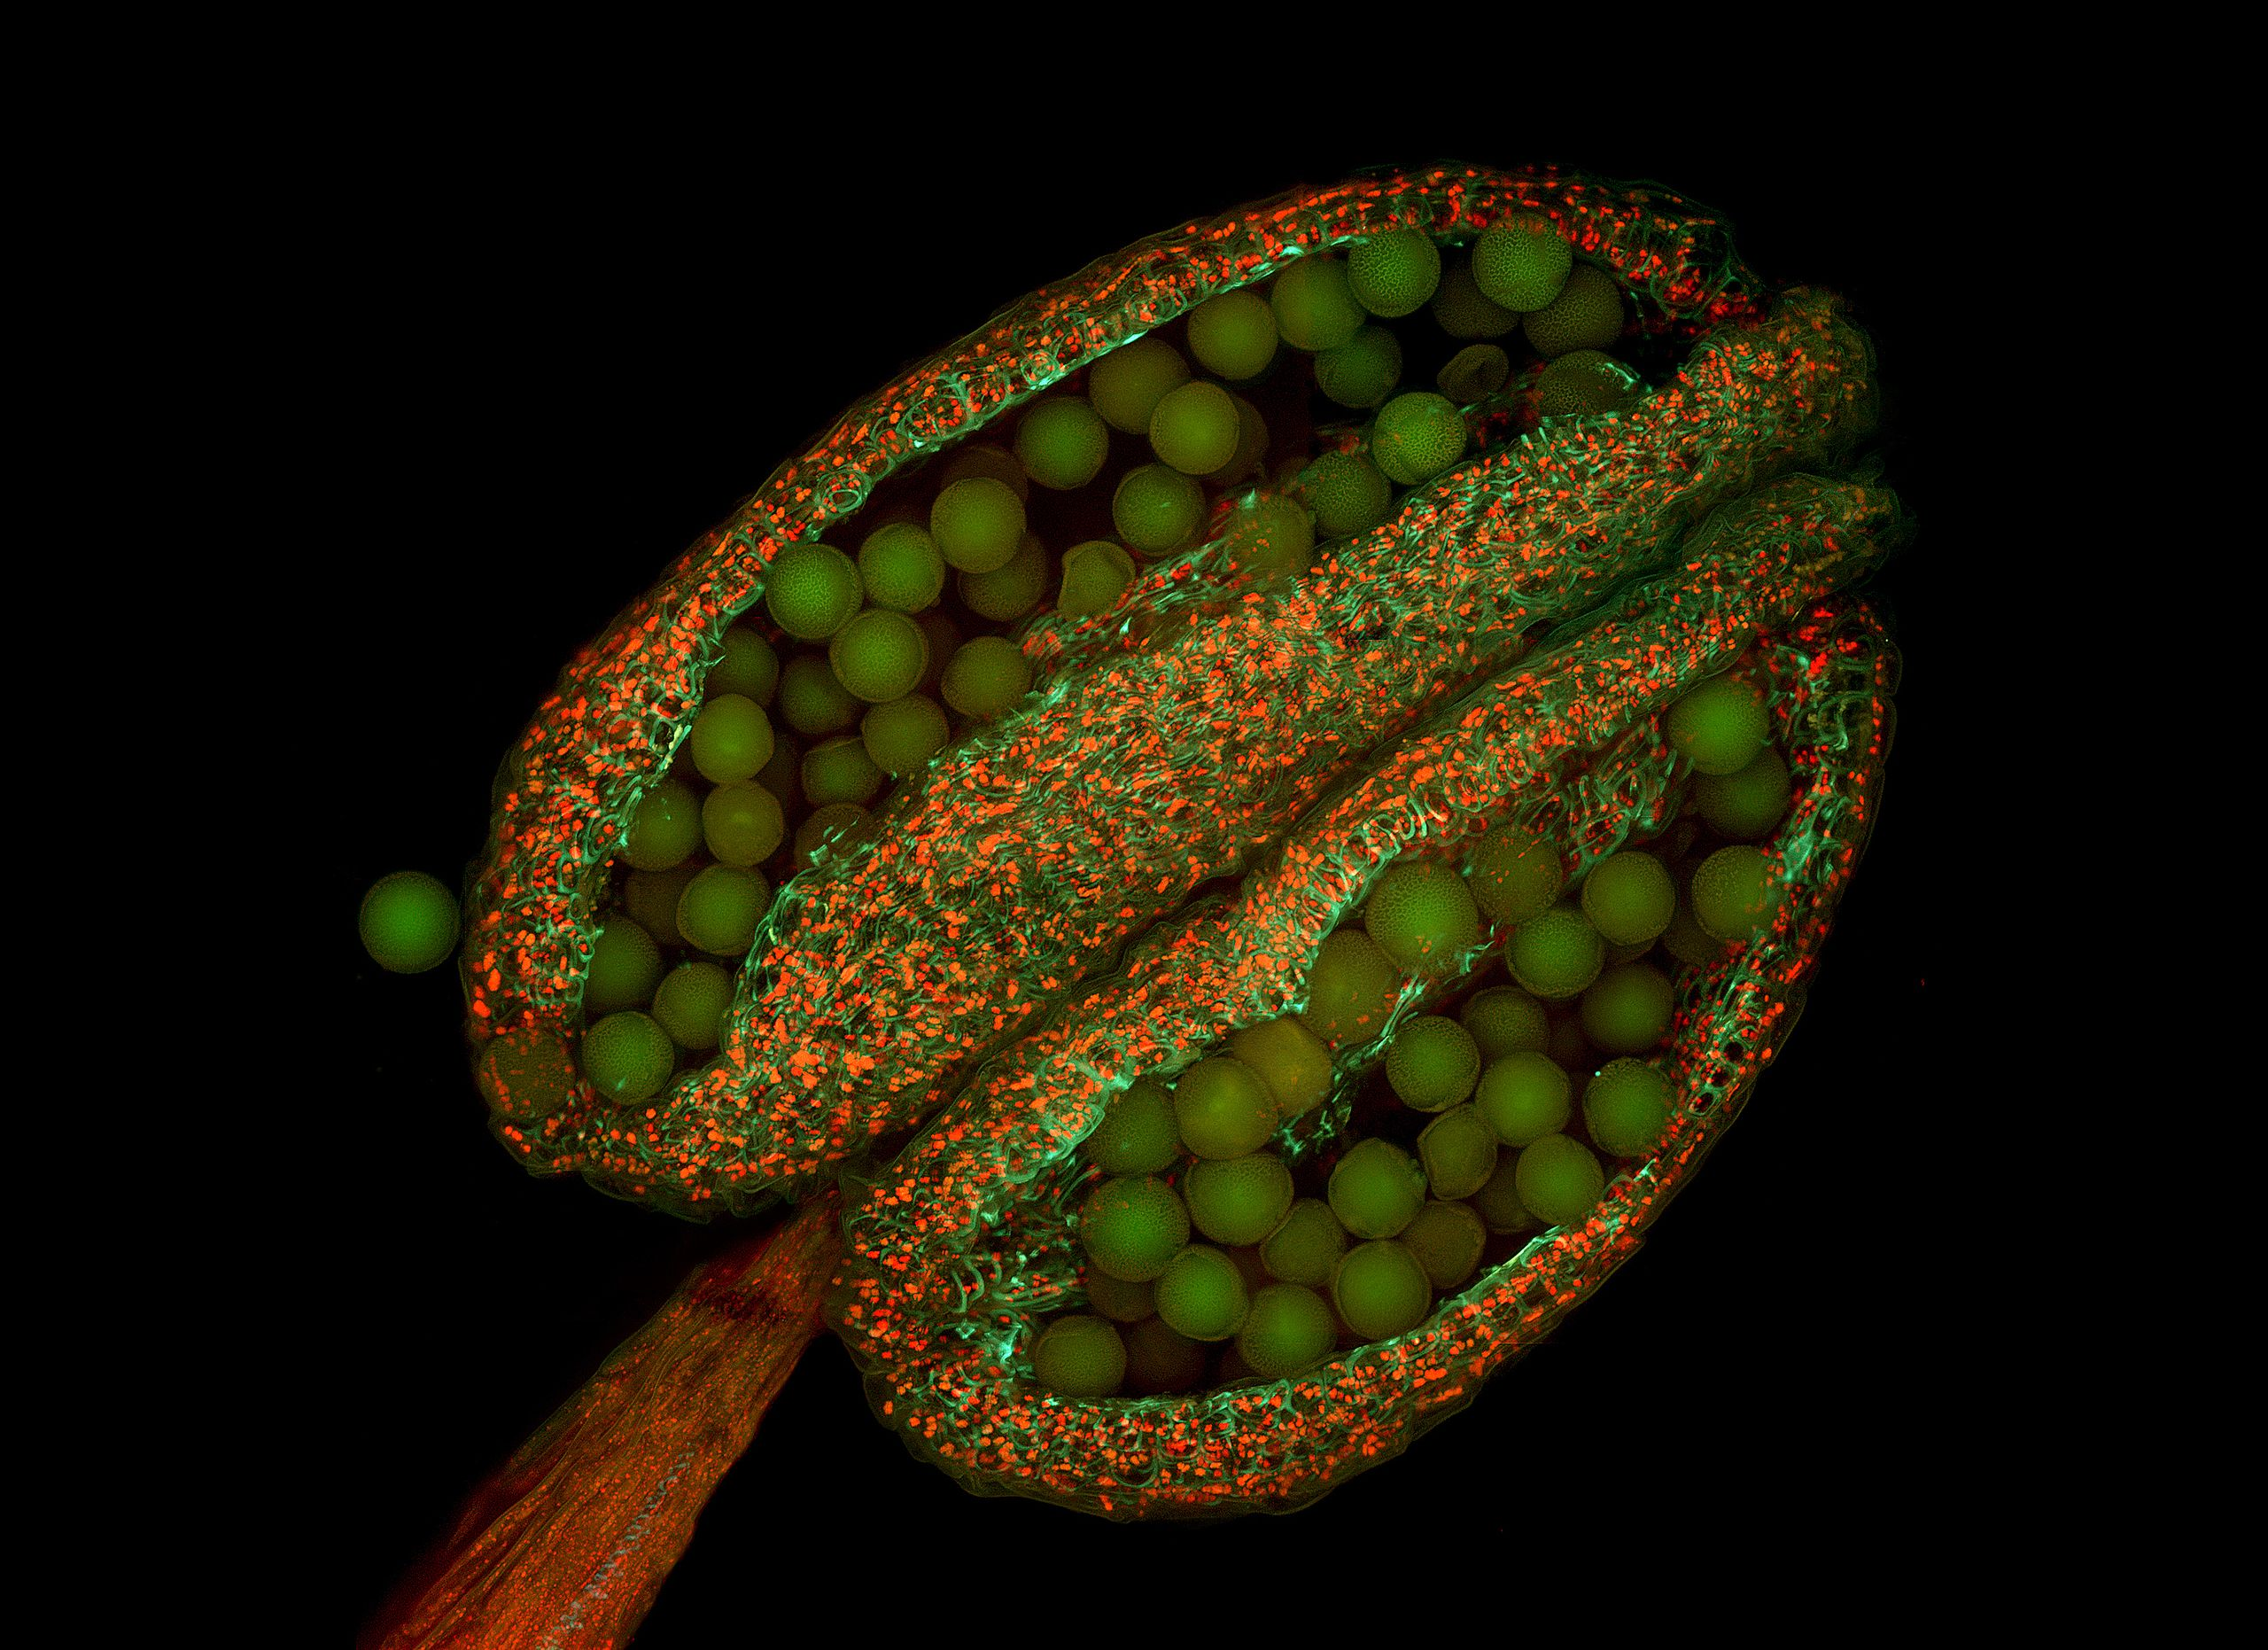
\includegraphics[width=\linewidth]{Tolmukapea.jpg}
	\caption{Anther of thale cress (Arabidopsis thaliana), fluorescence micrograph. Source: Heiti Paves, \href{https://commons.wikimedia.org/wiki/File:Tolmukapea.jpg}{https://commons.wiki-\\media.org/wiki/File:Tolmukapea.jpg}.}
	\label{fig:tcanther}
\end{figure}

Referencing a figure using its label: Figure \ref{fig:tcanther}.

Aenean porttitor eros non pharetra congue. Proin in odio in dolor luctus auctor ac et mi. Etiam euismod mi sed lectus fringilla pretium. Phasellus tristique maximus lectus et sodales. Mauris feugiat ligula quis semper luctus. Nam sit amet felis sed leo fermentum aliquet. Mauris arcu dui, posuere id sem eget, cursus pulvinar mi. Donec nec lacus non lectus fermentum scelerisque et at nibh. Sed tristique, metus ac vestibulum porta, tortor lectus placerat lorem, et convallis tellus dolor eget ante. Pellentesque dui ligula, hendrerit a purus et, volutpat tempor lectus. Mauris nec purus nec mauris rhoncus pellentesque. Quisque quis diam sed est lacinia congue. Donec magna est, hendrerit sed metus vel, accumsan rutrum nibh.

\begin{figure*} % Two column figure (notice the starred environment)
	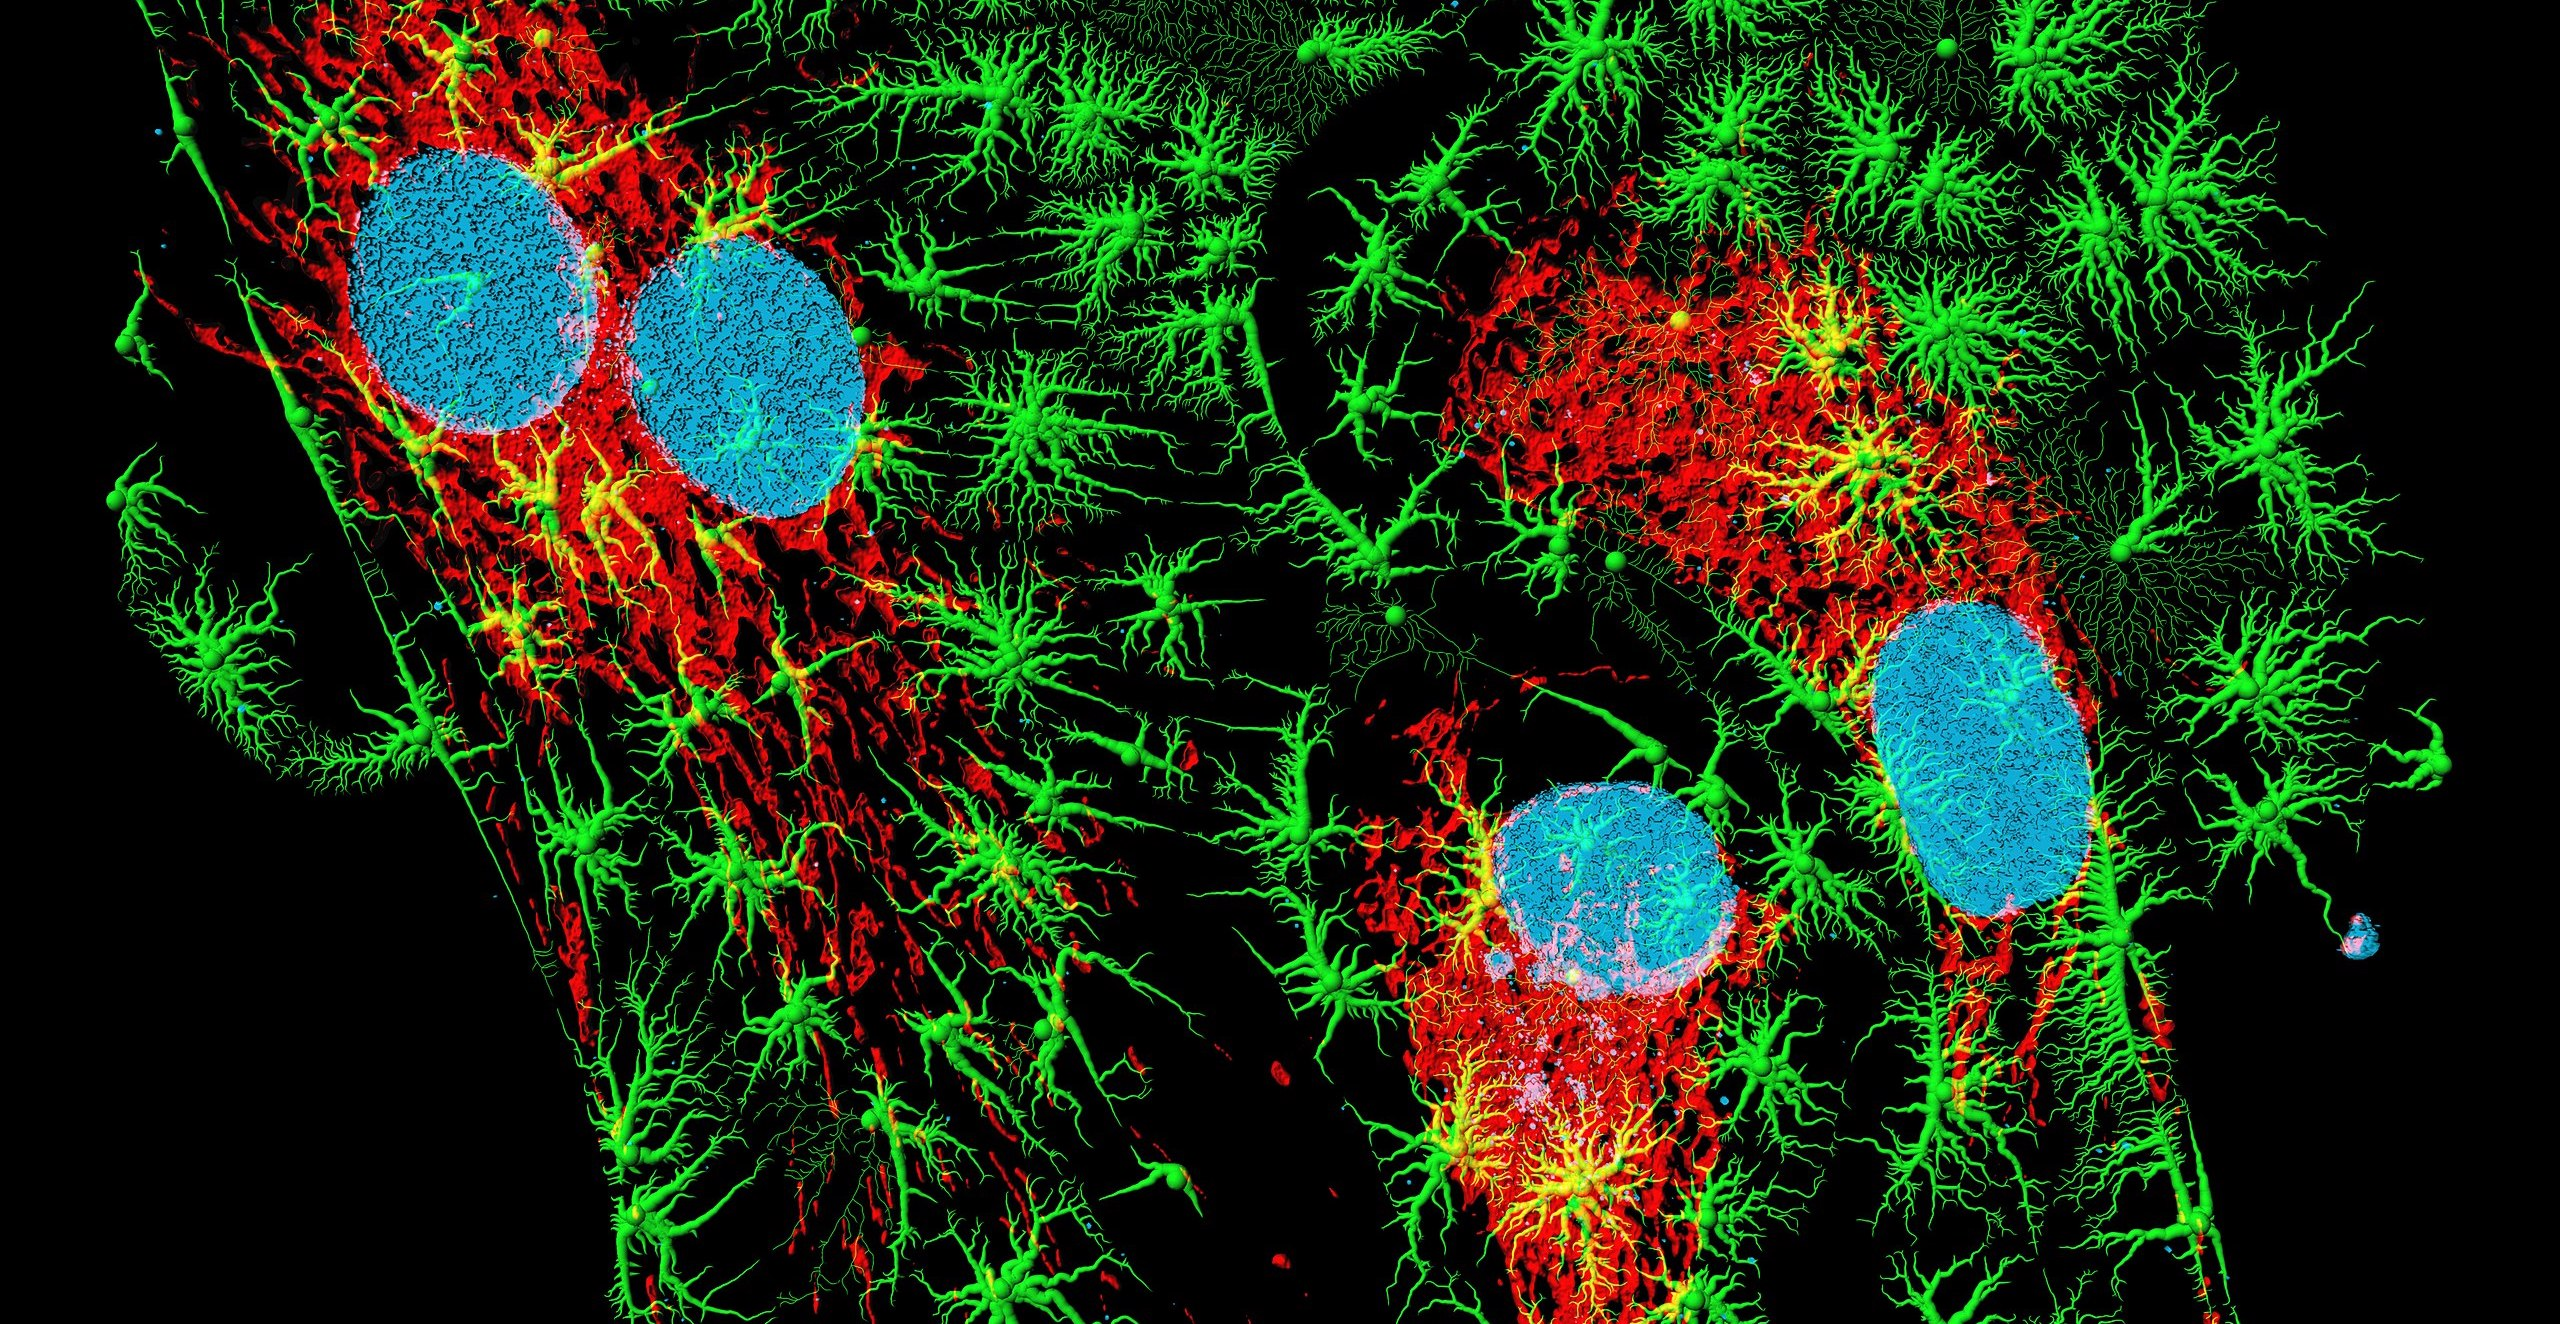
\includegraphics[width=\linewidth]{Fibroblastid.jpg}
	\caption{Bovine pulmonary artery endothelial cells in culture. Blue: nuclei; red: mitochondria; green: microfilaments. Computer generated image from a 3D model based on a confocal laser scanning microscopy using fluorescent marker dyes. Source: Heiti Paves, \href{https://commons.wikimedia.org/wiki/File:Fibroblastid.jpg}{https://commons.wikimedia.org/wiki/File:Fibroblastid.jpg}.}
	\label{fig:bpartery}
\end{figure*}

Orci varius natoque penatibus et magnis dis parturient montes, nascetur ridiculus mus. Etiam cursus lectus purus, tempus iaculis quam dictum tristique. Nam interdum sapien nec tempor mattis. Quisque id sapien nisi. Mauris vehicula ornare eros vel efficitur. Nulla consectetur, turpis quis fringilla tincidunt, mi neque iaculis lectus, vel commodo elit odio non ex. Duis facilisis, purus ac viverra iaculis, turpis lectus ultrices ante, ac vestibulum ligula magna in libero. Etiam tristique maximus lacinia. Vestibulum hendrerit, lacus malesuada laoreet blandit, sapien velit sollicitudin nunc, eu porttitor urna ligula at lorem. Aliquam faucibus eros in fermentum venenatis. Fusce consectetur congue pellentesque. Suspendisse at nisi sit amet est porttitor cursus. Cras placerat faucibus nunc, a laoreet justo dignissim sit amet.

\subsection{International Support}

\noindent àáâäãåèéêëìíîïòóôöõøùúûüÿýñçčšž

\noindent ÀÁÂÄÃÅÈÉÊËÌÍÎÏÒÓÔÖÕØÙÚÛÜŸÝÑ

\noindent ßÇŒÆČŠŽ

\subsection{Links}

This is a clickable URL link: \href{https://www.latextemplates.com}{LaTeX Templates}. This is a clickable email link: \href{mailto:vel@latextemplates.com}{vel@latextemplates.com}. This is a clickable monospaced URL link: \url{https://www.LaTeXTemplates.com}.

%------------------------------------------------

\section{Discussion}

This statement requires citation \autocite{Smith:2023qr}. This statement requires multiple citations \autocite{Smith:2023qr, Smith:2024jd}. This statement contains an in-text citation, for directly referring to a citation like so: \textcite{Smith:2024jd}.

\subsection{Subsection One}

Suspendisse potenti. Vivamus suscipit dapibus metus. Proin auctor iaculis ex, id fermentum lectus dapibus tristique. Nullam maximus eros eget leo pretium dapibus. Nunc in auctor erat, id interdum risus. Suspendisse aliquet vehicula accumsan. In vestibulum efficitur dictum. Sed ultrices, libero nec fringilla feugiat, elit massa auctor ligula, vehicula tempor ligula felis in lectus. Suspendisse sem dui, pharetra ut sodales eu, suscipit sit amet felis. Donec pretium viverra ante, ac pulvinar eros. Suspendisse gravida consectetur urna. Pellentesque vitae leo porta, imperdiet eros eget, posuere sem. Praesent eget leo efficitur odio bibendum condimentum sit amet vel ex. Nunc maximus quam orci, quis pulvinar nibh eleifend ac. Quisque consequat lacus magna, eu posuere tellus iaculis ac. Sed vitae tortor tincidunt ante sagittis iaculis.

\subsection{Subsection Two}

Nullam mollis tellus lorem, sed congue ipsum euismod a. Donec pulvinar neque sed ligula ornare sodales. Nulla sagittis vel lectus nec laoreet. Nulla volutpat malesuada turpis at ultricies. Ut luctus velit odio, sagittis volutpat erat aliquet vel. Donec ac neque eget neque volutpat mollis. Vestibulum viverra ligula et sapien bibendum, vel vulputate ex euismod. Curabitur nec velit velit. Aliquam vulputate lorem elit, id tempus nisl finibus sit amet. Curabitur ex turpis, consequat at lectus id, imperdiet molestie augue. Curabitur eu eros molestie purus commodo hendrerit. Quisque auctor ipsum nec mauris malesuada, non fringilla nibh viverra. Quisque gravida, metus quis semper pulvinar, dolor nisl suscipit leo, vestibulum volutpat ante justo ultrices diam. Sed id facilisis turpis, et aliquet eros.

\subsubsection{Subsubsection Example}

Duis venenatis eget lectus a aliquet. Integer vulputate ante suscipit felis feugiat rutrum. Aliquam eget dolor eu augue elementum ornare. Nulla fringilla interdum volutpat. Sed tincidunt, neque quis imperdiet hendrerit, turpis sapien ornare justo, ac blandit felis sem quis diam. Proin luctus urna sit amet felis tincidunt, sed congue nunc pellentesque. Ut faucibus a magna faucibus finibus. Etiam id mi euismod, auctor nisi eget, pretium metus. Proin tincidunt interdum mi non interdum. Donec semper luctus dolor at elementum. Aenean eu congue tortor, sed hendrerit magna. Quisque a dolor ante. Mauris semper id urna id gravida. Vestibulum mi tortor, finibus eu felis in, vehicula aliquam mi.

Aliquam arcu turpis, ultrices sed luctus ac, vehicula id metus. Morbi eu feugiat velit, et tempus augue. Proin ac mattis tortor. Donec tincidunt, ante rhoncus luctus semper, arcu lorem lobortis justo, nec convallis ante quam quis lectus. Aenean tincidunt sodales massa, et hendrerit tellus mattis ac. Sed non pretium nibh. 

Donec cursus maximus luctus. Vivamus lobortis eros et massa porta porttitor. Nam vitae suscipit mi. Pellentesque ex tellus, iaculis vel libero at, cursus pretium sapien. Curabitur accumsan velit sit amet nulla lobortis, ut pretium ex aliquam. Proin eget volutpat orci. Morbi eu aliquet turpis. Vivamus molestie urna quis tempor tristique. Proin hendrerit sem nec tempor sollicitudin.

%----------------------------------------------------------------------------------------
%	 REFERENCES
%----------------------------------------------------------------------------------------

\printbibliography % Output the bibliography

%----------------------------------------------------------------------------------------

\end{document}
